%! TeX program = xelatex
\documentclass{note}

\begin{document}
%%%%%%%%%%%%%%%%%%%%%%%%%%%%%%%%%%%%%%%%%%%%%%%%%%%%%%%%%%%%%%%%%%%%%%%%%%%%
%                               COVER
%%%%%%%%%%%%%%%%%%%%%%%%%%%%%%%%%%%%%%%%%%%%%%%%%%%%%%%%%%%%%%%%%%%%%%%%%%%%    
% 参考https://tex.stackexchange.com/questions/23766/suppress-fancy-header-and-footer-on-first-page-only
% 参考https://tex.stackexchange.com/questions/57158/centered-title-page-in-twoside-report
% Cover page
\clearpage
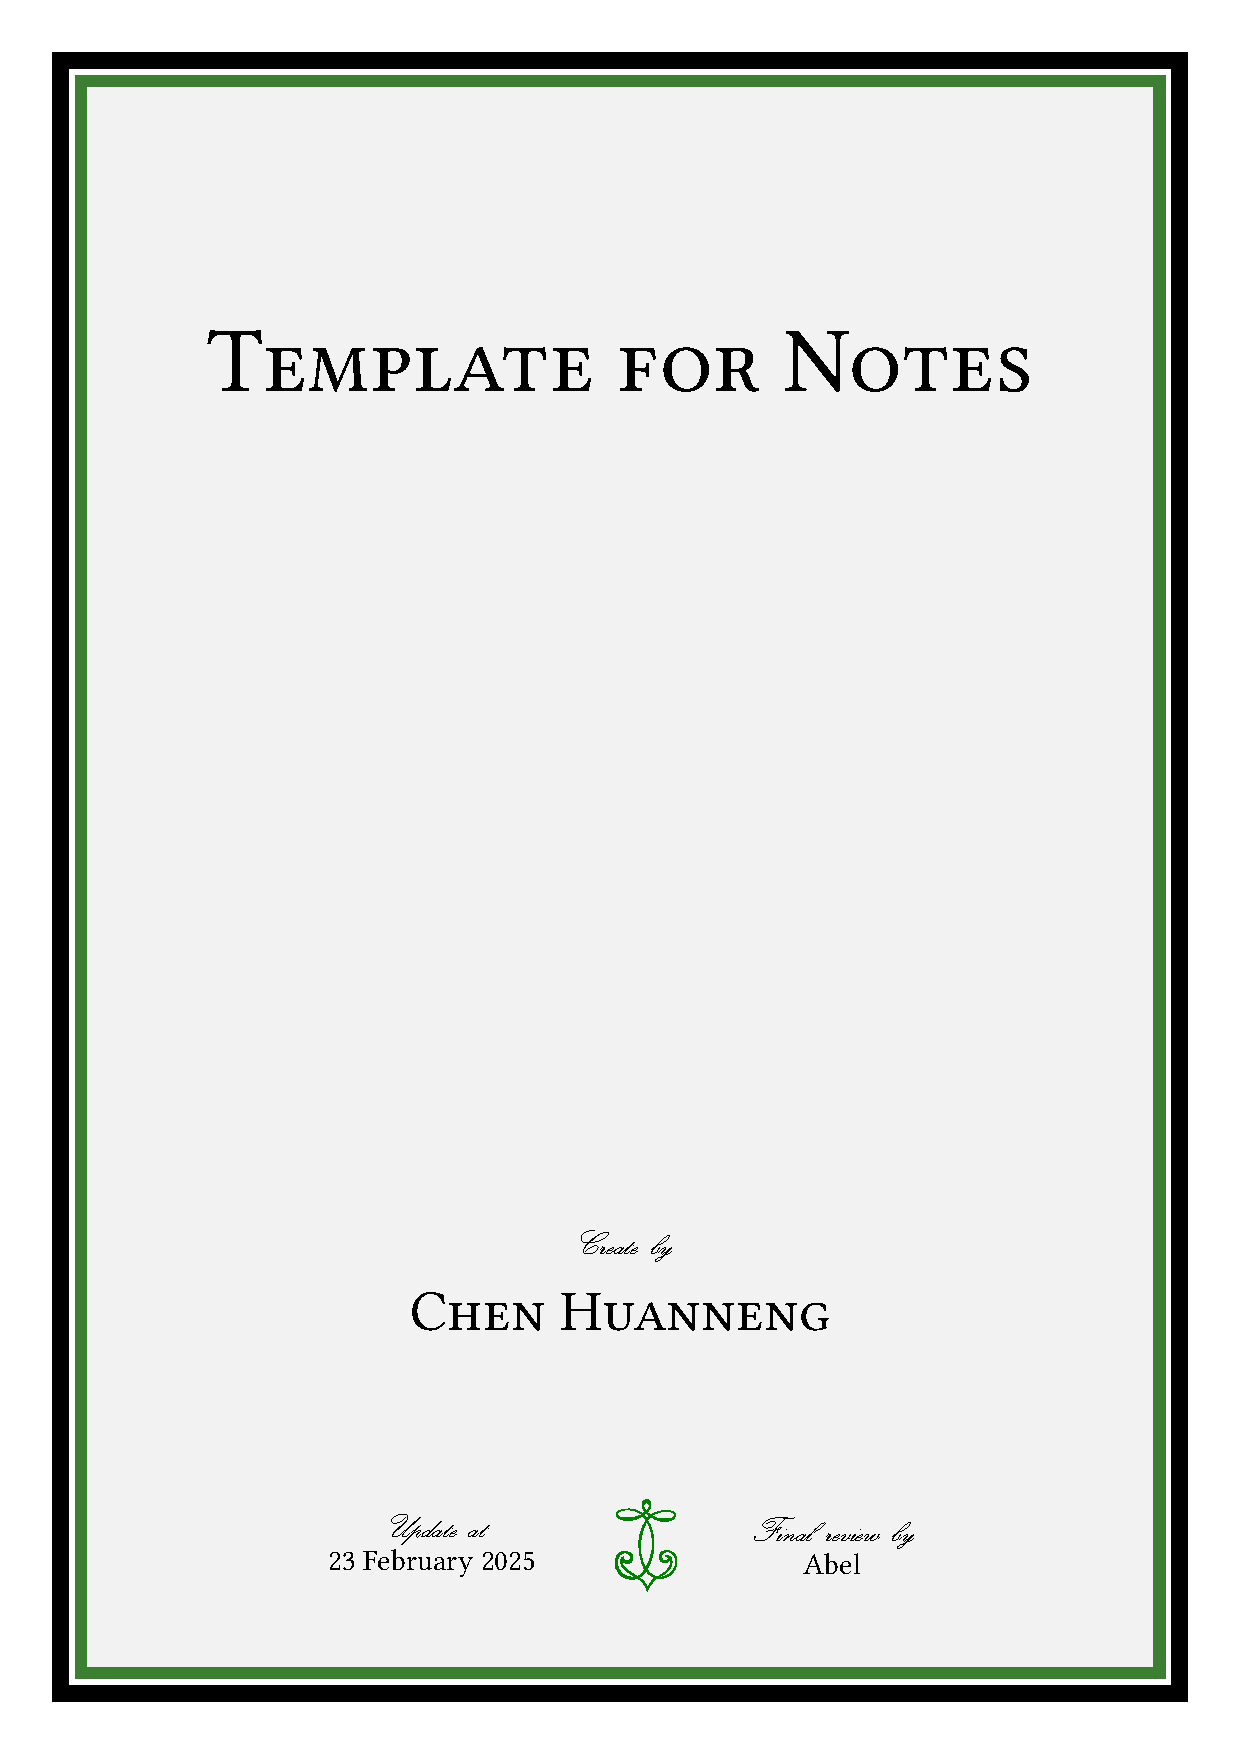
\includepdf{cover/cover.pdf}
\thispagestyle{empty}
\clearpage

% Title page
\begin{titlepage}
\thispagestyle{empty} % 清除页脚页眉
\noindent
\titlefont Template for note\par
\epigraph{Pure mathematics is on the whole distinctly more useful than applied. For what is useful above all is technique, and mathematical technique is taught mainly through pure mathematics.}%
{\textit{London 1941}\\ \textsc{G. H. Hardy}}
\null\vfill
\vspace*{1cm}
\noindent
\hfill
\begin{minipage}{0.5\linewidth}
    \begin{flushright}
        \printauthor
    \end{flushright}
\end{minipage}
%
\begin{minipage}{0.02\linewidth}
    \rule{1pt}{60pt}
\end{minipage}
\titlepagedecoration

% 增加空白页方便打印
% 参考https://tex.stackexchange.com/questions/508315/add-unnumbered-blank-page-after-cover-page-but-before-title-page-and-book
\clearpage
~
\thispagestyle{empty}
\clearpage

\end{titlepage}

%%%%%%%%%%%%%%%%%%%%%%%%%%%%%%%%%%%%%%%%%%%%%%%%%%%%%%%%%%%%%%%%%%%%%%%%%%%%
%                           TABLE OF CONTENTS
%%%%%%%%%%%%%%%%%%%%%%%%%%%%%%%%%%%%%%%%%%%%%%%%%%%%%%%%%%%%%%%%%%%%%%%%%%%%
% 生成目录
{
    \pagenumbering{Alph} % 目录页码编号为大写字母
    \hypersetup{linkcolor=red!65!black} % 设置局部目录超链接颜色
    \tableofcontents
}

%%%%%%%%%%%%%%%%%%%%%%%%%%%%%%%%%%%%%%%%%%%%%%%%%%%%%%%%%%%%%%%%%%%%%%%%%%%%
%                            FRONTMATTER
%%%%%%%%%%%%%%%%%%%%%%%%%%%%%%%%%%%%%%%%%%%%%%%%%%%%%%%%%%%%%%%%%%%%%%%%%%%%
\frontmatter

% \input{frontmatter}

\chapter{Frontmatter}
\lipsum[5-10]

%%%%%%%%%%%%%%%%%%%%%%%%%%%%%%%%%%%%%%%%%%%%%%%%%%%%%%%%%%%%%%%%%%%%%%%%%%%%
%                            MAINMATTER
%%%%%%%%%%%%%%%%%%%%%%%%%%%%%%%%%%%%%%%%%%%%%%%%%%%%%%%%%%%%%%%%%%%%%%%%%%%%
\mainmatter

% 每个章节就是一个.tex文件,方便后续的调试
% \input{chapter1}
% \input{chapter2}
% \input{chapter3}
% \input{chapter4}
% \input{chapter5}
% \input{chapter6}

\part{First Part}

\chapter{Introduction}

\section{Section 1.1}

hello world!\cite{2015The} This is a test text line.\url{https://github.com/chen-huaneng} And this is another test text line.\href{https://github.com/chen-huaneng}{Github} Also a test text line.\hyperref[test]{Subsection 1.1.1}

\lipsum[5-10]

\subsection{Subsection 1.1.1}\label{test}

\lipsum[5-10]

\part{Second Part}

\chapter{Column Generation}

\lipsum[5-10]

\section{Section 2.1}

\lipsum[5-10]

%%%%%%%%%%%%%%%%%%%%%%%%%%%%%%%%%%%%%%%%%%%%%%%%%%%%%%%%%%%%%%%%%%%%%%%%%%%%
%                            BACKMATTER
%%%%%%%%%%%%%%%%%%%%%%%%%%%%%%%%%%%%%%%%%%%%%%%%%%%%%%%%%%%%%%%%%%%%%%%%%%%%
\backmatter

% \input{appendix}

%%%%%%%%%%%%%%%%%%%%%%%%%%%%%%%%%%%%%%%%%%%%%%%%%%%%%%%%%%%%%%%%%%%%%%%%%%%%
%                            APPENDIX
%%%%%%%%%%%%%%%%%%%%%%%%%%%%%%%%%%%%%%%%%%%%%%%%%%%%%%%%%%%%%%%%%%%%%%%%%%%%
\chapter*{Appendix}
% \addcontentsline{toc}{chapter}{Appendix}
\chaptermark{Appendix}

\lipsum[5-10]

\section*{Hello World}
\sectionmark{Hello World}

\lipsum[10-20]

\section{Section}

\lipsum[5-10]

%%%%%%%%%%%%%%%%%%%%%%%%%%%%%%%%%%%%%%%%%%%%%%%%%%%%%%%%%%%%%%%%%%%%%%%%%%%%
%                            REFERENCES
%%%%%%%%%%%%%%%%%%%%%%%%%%%%%%%%%%%%%%%%%%%%%%%%%%%%%%%%%%%%%%%%%%%%%%%%%%%%
\bibliography{references}

\end{document}
